\subsection{Hyperbolic space}
From the visual standpoint, the hyperbolic space can be identified by the fact that the otherwise flat terrain appears "curved downward".
This may create an illusion that the terrain is wrapped around a giant sphere.
\todo{That's at least how it looks to me}
However, by exploring the hyperbolic space, we can quickly notice that it is infinite, just like the Euclidean space.
\autoref{fig:hyperbolic-space-games} shows the comparison of the depictions of hyperbolic space between our game and \textit{Hyperbolica}.
\begin{figure*}[h]
    \centering
    \begin{subfigure}[b]{0.475\textwidth}
        \centering
        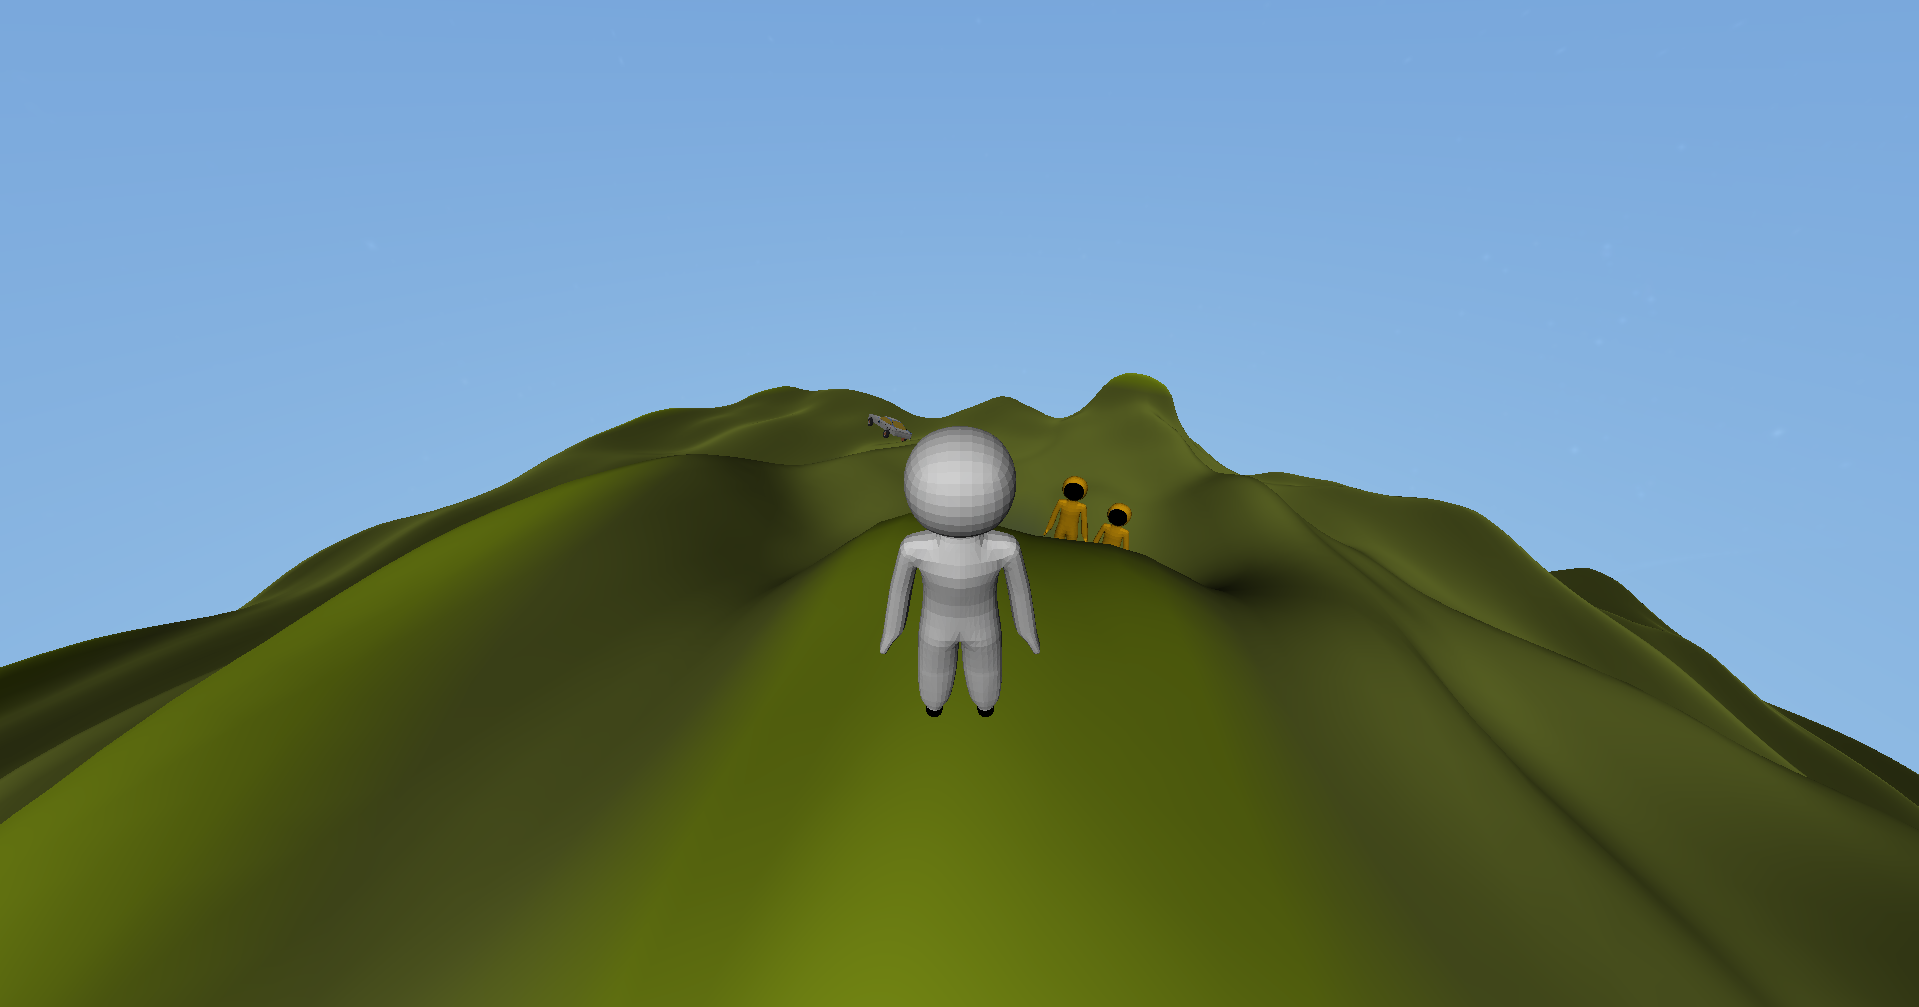
\includegraphics[width=\textwidth]{chapters/results/sections/non_euclidean/resources/hyperbolic-in-hyper.png}
        \caption[]%
        {{\small \textit{Hyper}}}
        \label{fig:hyperbolic-space-games-hyper}
    \end{subfigure}
    \hfill
    \begin{subfigure}[b]{0.475\textwidth}
        \centering
        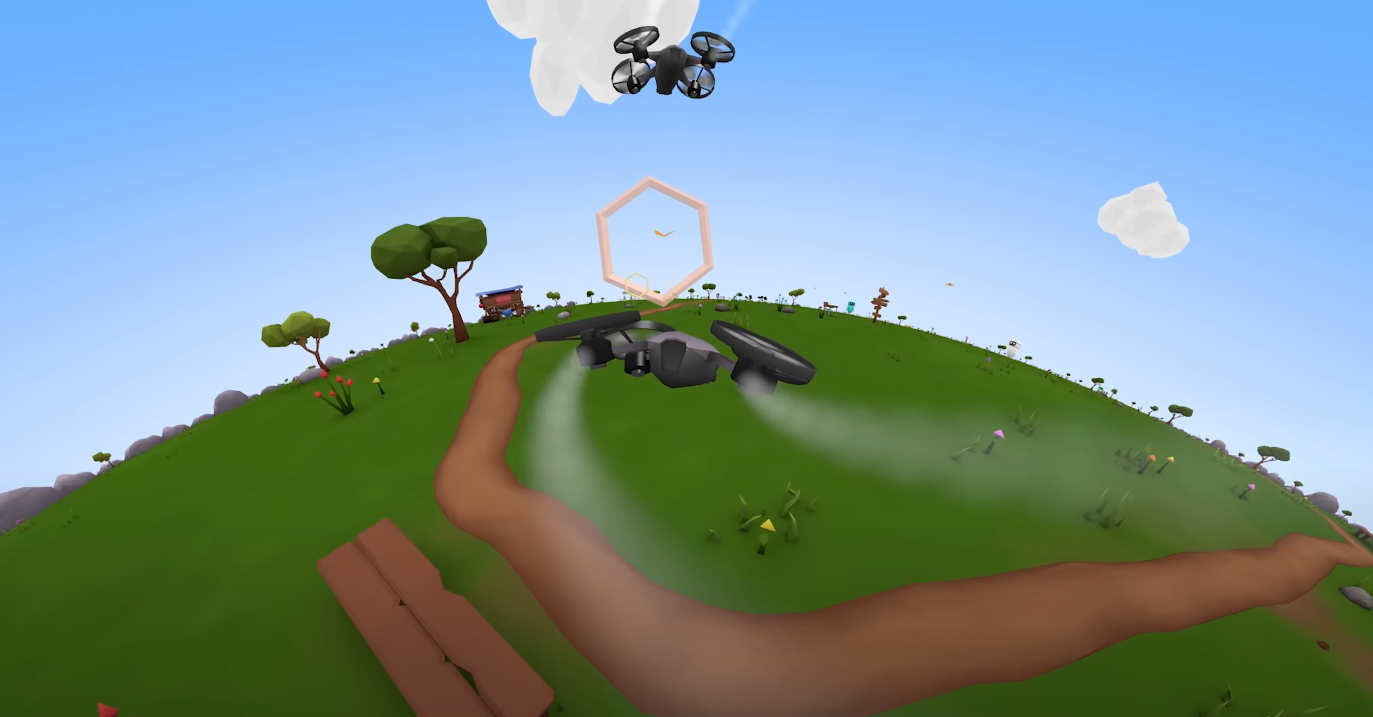
\includegraphics[width=\textwidth]{chapters/results/sections/non_euclidean/resources/hyperbolica-hyperbolic.png}
        \caption[]%
        {{\small \textit{Hyperbolica \cite{Hyperbolica-Hyperbolic}}}}
        \label{fig:hyperbolic-space-games-hyperbolica}
    \end{subfigure}
    \caption[]
    {\small Hyperbolic space}
    \label{fig:hyperbolic-space-games}
\end{figure*}

\todo{We have to mention that our non-Euclidean spaces are "fake" in the sense that you don't have 5-sided right pentagons and all that jazz.}